\section{Problem 3.2}

Given a Z channel with probabilities $p_{Y|X}(0|0)=1$, $p_{Y|X}(1|0)=0$, $p_{Y|X}(1|1)=p_{Y|X}(0|1)=\frac{1}{2}$, we want to find the channel capacity $C$. We know that the channel capacity for a discrete memory channel is defined as follows.

\begin{equation}
	C = \max_{p_X} I(X;Y) = H(Y)-H(Y|X)
\end{equation}

First we compute $H(Y)$ in function of $p=p_X(1)$.

\begin{equation}
\begin{aligned}
	H(Y)= & -p_Y(1)\cdot\log(p_Y(1))-p_Y(0)\cdot\log(p_Y(0)) \\
	= & -(p_{Y|X}(1|0) \cdot p_X(0) + p_{Y|X}(1|1) \cdot p_X(1)) \cdot\log(p_{Y|X}(1|0) \cdot p_X(0) + p_{Y|X}(1|1) \cdot p_X(1)) \\ & -(p_{Y|X}(0|0) \cdot p_X(0) + p_{Y|X}(0|1) \cdot p_X(1)) \cdot\log(p_{Y|X}(0|0) \cdot p_X(0) + p_{Y|X}(0|1) \cdot p_X(1)) \\
	= & -\frac{1}{2}\cdot p_X(1)\log\Big(\frac{1}{2}\cdot p_X(1)\Big)-\Big(p_X(0)+\frac{1}{2}\cdot p_X(1)\Big)\cdot \log \Big(p_X(0)+\frac{1}{2}\cdot p_X(1)\Big) \\
	= & -\frac{1}{2}\cdot p \cdot \log\Big(\frac{1}{2}\cdot p\Big)-\Big(1-\frac{1}{2}\cdot p\Big)\cdot \log \Big(1-\frac{1}{2}\cdot p\Big)
\end{aligned}
\end{equation}

Then we compute $H(Y|X)$ always in funcion of $p=p_X(1)$.

\begin{equation}
\begin{aligned}
	H(Y|X) = & -p_{YX}(0,0) \cdot \log (p_{Y|X}(0|0)) -p_{YX}(1,0) \cdot \log (p_{Y|X}(1|0)) \\
	& -p_{YX}(0,1) \cdot \log (p_{Y|X}(0|1)) -p_{YX}(1,1) \cdot \log (p_{Y|X}(1|1)) \\ =
	& -p_{Y|X}(0|0) \cdot p_X(0) \cdot \log (p_{Y|X}(0|0)) -p_{Y|X}(1|0) \cdot p_X(0) \cdot \log (p_{Y|X}(1|0)) \\
	& -p_{Y|X}(0|1) \cdot p_X(1) \cdot \log (p_{Y|X}(0|1)) -p_{Y|X}(1|1) \cdot p_X(1) \cdot \log (p_{Y|X}(1|1)) \\ =	& 0 + 0 + \frac{1}{2} \cdot p + \frac{1}{2} \cdot p = p
\end{aligned}
\end{equation}

Now we are able to write $I(X;Y)$ in function of $p$ as we can see from \eqref{IXY}.

\begin{equation}
	I(X;Y) = -\frac{1}{2}\cdot p \cdot \log\Big(\frac{1}{2}\cdot p\Big)-\Big(1-\frac{1}{2}\cdot p\Big)\cdot \log \Big(1-\frac{1}{2}\cdot p\Big)-p
	\label{IXY}
\end{equation}

\pagebreak

In \ref{fig:funcinfoex1} we show the function's trend for all possible values of $p$.

\begin{figure}[h!]
	\centering
	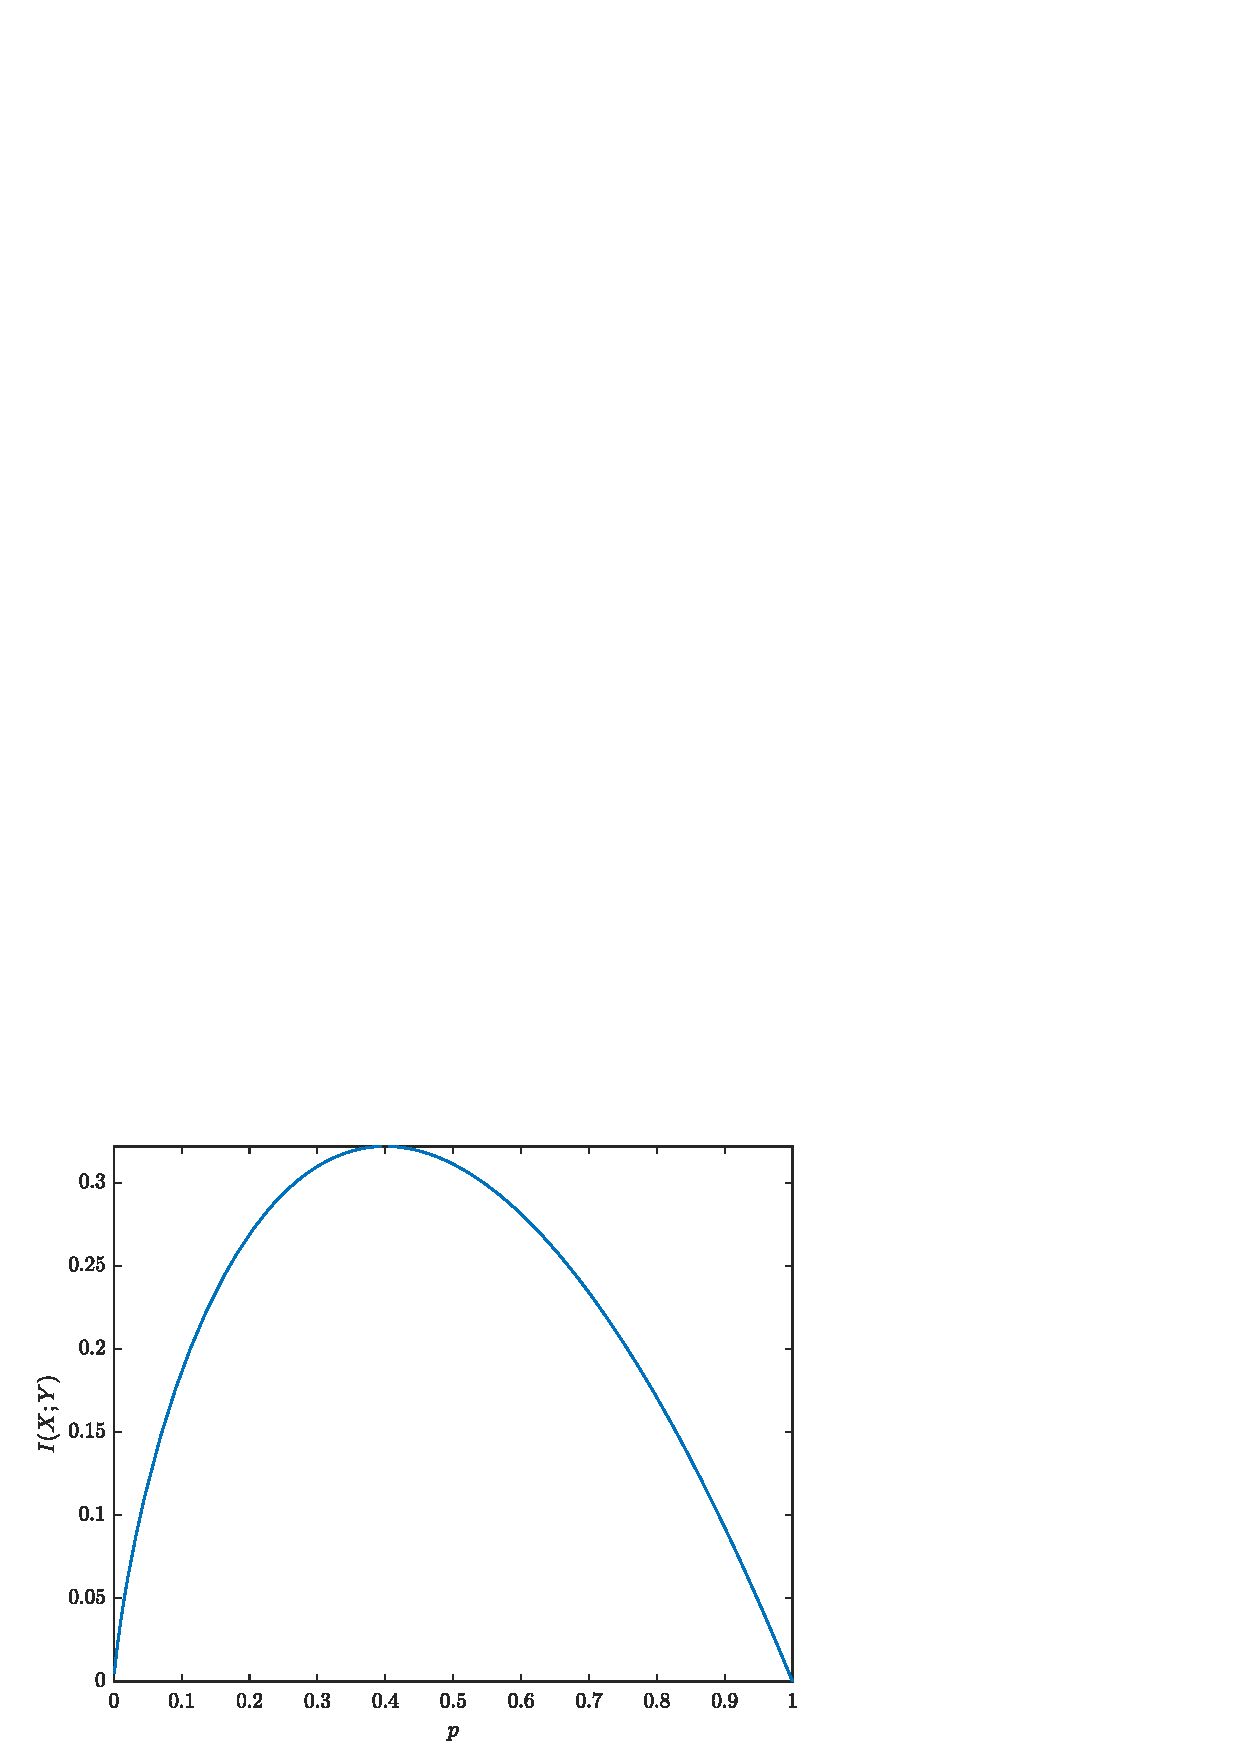
\includegraphics[width=0.7\linewidth]{img/func_info_ex1}
	\caption{Mutual information as a function of $p \triangleq p_X(1)$}
	\label{fig:funcinfoex1}
\end{figure}

Now we want to find the value of $p$ for which \eqref{IXY} is maximize. With this aim we compute the first and the second derivates of $I(X;Y)$.

\begin{equation}
\begin{aligned}
	\frac{dI(X;Y)}{dp}= &\frac{1}{2} \cdot \log \Big( 1 - \frac{p}{2}\Big)+ \frac{1}{2} \cdot \frac{1- \frac{p}{2}}{1-\frac{p}{2}} - \frac{1}{2} \cdot \log\Big ( \frac{p}{2}\Big)-\frac{p}{2} \cdot \frac{2}{p} \cdot \frac{1}{2} - 1 \\
	= & \frac{1}{2} \cdot \log \Big ( \frac{2}{p} - 1\Big)-1
	\end{aligned}
	\end{equation}

\begin{equation}
\begin{aligned}
	\frac{d^2I(X;Y)}{dp^2}= \frac{1}{2}\cdot \frac{p}{2-p} \cdot \frac{1}{2}= \frac{1}{4} \cdot \frac{p}{2-p}
\end{aligned}
\end{equation}

We notice that $\frac{d^2I(X;Y)}{dp^2}$ is always equal or greater than zero for every possibli value of p. This means that $I(X;Y)$ is a convex function and then the value of $p$ for which $\frac{dI(X;Y)}{dp}$ is zero coincides with the maximum point of $I(X;Y)$. Therefore we compute the values for which we have $\frac{dI(X;Y)}{dp}=0$.

\begin{equation}
\begin{gathered}
	\frac{1}{2} \cdot \log \Big ( \frac{2}{p} - 1\Big)-1 = 0 \\
	\log \Big ( \frac{2}{p} - 1\Big) = 2 \\
	\frac{2}{p} - 1 = 2^2 \\
	p = \frac{2}{5}
\end{gathered}
\end{equation}

So for $p=\frac{2}{5}$ we maximize $I(X;Y)$ and therefore we obtain the value of the channel capacity $C$. The value of $C$ is reported in \eqref{C}.

\begin{equation}
\begin{aligned}
	C = & I(X;Y)|_{p=\frac{2}{5}} \\ = &-\frac{4}{5} \cdot \log\Big (\frac{4}{5}\Big)- \frac{1}{5}\cdot\log \Big(\frac{1}{5}\Big)-\frac{2}{5} \\
	= & \frac{1}{5} \cdot \log \Big (\frac{3125}{256} \Big)-\frac{2}{5}
	\label{C}
\end{aligned}
\end{equation}
